\documentclass[aspectratio=169, 10pt]{beamer}

% =========================================================================
% MINIMALIST BEIGE & NAVY THEME
% Background: #F3EBE1 (Warm Cream Beige) | Typography: #262E5B (Deep Indigo Navy)
% Biên dịch bằng XeLaTeX hoặc LuaLaTeX (KHÔNG dùng pdfLaTeX vì có fontspec)
% =========================================================================

\usetheme{default}
\setbeamertemplate{navigation symbols}{}
\setbeamertemplate{headline}{}
\setbeamertemplate{footline}{}

\usepackage{fontspec}
% [SỬA LỖI 1] Segoe UI chỉ có trên Windows -> máy khác/Overleaf báo "font not found".
% Tự động dùng font dự phòng nếu không có Segoe UI.
\IfFontExistsTF{Segoe UI}{\setsansfont{Segoe UI}\setmainfont{Segoe UI}}{%
  \IfFontExistsTF{Carlito}{\setsansfont{Carlito}\setmainfont{Carlito}}{%
    \setsansfont{DejaVu Sans Condensed}\setmainfont{DejaVu Sans Condensed}}}

\usepackage{graphicx}
\usepackage{booktabs}
\usepackage{amsmath,amssymb}
\usepackage{xcolor}
\usepackage{tikz}
\usetikzlibrary{calc,positioning,shapes.geometric,arrows.meta}

% --- COLOR DEFINITIONS ---
\definecolor{bgBeige}{RGB}{243, 235, 225}
\definecolor{navyMain}{RGB}{38, 46, 91}
\definecolor{navyMuted}{RGB}{85, 95, 140}
\definecolor{navyLight}{RGB}{228, 225, 235}
\definecolor{accentDark}{RGB}{185, 28, 28}
\definecolor{boxBg}{RGB}{230, 221, 208}
\definecolor{accentRed}{RGB}{185, 28, 28}

\setbeamercolor{background canvas}{bg=bgBeige}
\setbeamercolor{normal text}{fg=navyMain}
\setbeamercolor{structure}{fg=navyMain}

\setbeamersize{text margin left=1.0cm, text margin right=1.8cm}

% --- BACKGROUND WITH RIGHT NAVY ACCENT BAR ---
\setbeamertemplate{background}{
    \begin{tikzpicture}[remember picture,overlay]
        \fill[bgBeige] (current page.south west) rectangle (current page.north east);
        \fill[navyMain, rounded corners=16pt]
            ($(current page.north east)+(-1.05cm, 0)$) rectangle ($(current page.south east)+(1.0cm, 0)$);
    \end{tikzpicture}
}

% --- SLIDE HEADER ---
\newcommand{\slideheader}[2]{%
    \vspace*{-0.15cm}%
    {\fontsize{7.5pt}{9pt}\selectfont \textbf{\color{navyMuted}\MakeUppercase{#1}}}\\[0.03cm]
    {\fontsize{13.5pt}{16pt}\selectfont \textbf{\color{navyMain}\MakeUppercase{#2}}}\\[0.08cm]
}

% --- FOOTER + SỐ TRANG ---
\newcommand{\slidenumber}[1]{%
    \begin{tikzpicture}[remember picture,overlay]
        \node[anchor=south east] at ($(current page.south east)+(-1.4cm, 0.35cm)$) {
            \textcolor{navyMuted}{\fontsize{8.5pt}{10pt}\selectfont \textbf{\insertframenumber}}
        };
        \node[anchor=south west] at ($(current page.south west)+(1.0cm, 0.35cm)$) {
            \textcolor{navyMuted}{\fontsize{7pt}{8pt}\selectfont \textit{Hands-On Data Visualization} -- Jack Dougherty \& Ilya Ilyankou}
        };
    \end{tikzpicture}%
}

% --- CALLOUT BOX ---
\newcommand{\calloutbox}[3][\textwidth]{%
    \begin{tikzpicture}
        \node[fill=boxBg, draw=navyMain, line width=0.8pt, rounded corners=4pt,
              inner sep=5pt, text width=#1-14pt, align=left] {
            {\fontsize{8.5pt}{10.5pt}\selectfont \textbf{\color{navyMain}#2}}\\[0.03cm]
            {\fontsize{7.5pt}{9.5pt}\selectfont \color{navyMain}#3}
        };
    \end{tikzpicture}%
}

% --- PILL BOX ---
\newcommand{\pillbox}[2][]{%
    \begin{tikzpicture}
        \node[draw=navyMain, rounded corners=10pt, line width=1.1pt,
              inner xsep=12pt, inner ysep=4pt, text=navyMain, #1] {\textbf{#2}};
    \end{tikzpicture}%
}

% [SỬA LỖI 2] Thiếu file ảnh trong images/ -> lỗi "File not found" và dừng biên dịch.
% Nếu ảnh có thật: chèn bình thường. Nếu chưa có: vẽ khung giữ chỗ cùng kích thước.
\pgfkeys{/ph/.is family, /ph,
  width/.store in=\phw, height/.store in=\phh, .unknown/.code={}}
\let\origincludegraphics\includegraphics
\renewcommand{\includegraphics}[2][]{%
  \IfFileExists{#2}{\origincludegraphics[#1]{#2}}{%
    \begingroup
    \pgfkeys{/ph, width=\linewidth, height=0.4\textheight, #1}%
    \begin{tikzpicture}
      \node[draw=navyMuted, dashed, line width=0.7pt, fill=white!55!bgBeige, rounded corners=3pt,
            minimum width=\phw, minimum height={0.8*(\phh)}, text width={\phw-8pt}, align=center,
            font=\fontsize{6pt}{7.5pt}\selectfont, text=navyMuted]
        {\textbf{[Chèn ảnh]}\\\detokenize{#2}};
    \end{tikzpicture}%
    \endgroup}}

\begin{document}

% ==================== SLIDE 1: TRANG BÌA ====================
\begin{frame}[plain, c]
\begin{tikzpicture}[remember picture,overlay]
    \node[anchor=north west] at ($(current page.north west)+(1.0cm, -0.8cm)$) {
        \textcolor{navyMuted}{\fontsize{8.5pt}{10.5pt}\selectfont Tháng 10, 2026}
    };
    \node[anchor=west, text width=0.84\textwidth] at ($(current page.west)+(1.0cm, 0.3cm)$) {
        {\fontsize{13pt}{15pt}\selectfont \textbf{\color{navyMuted} PHẦN 1 • BÁO CÁO CHUYÊN ĐỀ}}\\[0.25cm]
        {\fontsize{29pt}{33pt}\selectfont \textbf{\color{navyMain} NỀN TẢNG DỮ LIỆU}}\\[0.12cm]
        {\fontsize{20pt}{24pt}\selectfont \textbf{\color{navyMain} THU THẬP, LÀM SẠCH \& CHUẨN HÓA}}\\[0.35cm]
        \pillbox{\fontsize{9.5pt}{11.5pt}\selectfont Từ Dữ Liệu Thô Đến Phép So Sánh Công Bằng (Chương 3, 4, 5)}\\[0.45cm]
        {\fontsize{8.5pt}{10.5pt}\selectfont \color{navyMuted} Thuyết trình: \textbf{Trần Thị Mai Anh} • Tác phẩm: \textit{Hands-On Data Visualization} (Jack Dougherty \& Ilya Ilyankou)}
    };
\end{tikzpicture}
\slidenumber{01}
\end{frame}
% ==================== SLIDE 4: TRIẾT LÝ DỮ LIỆU KHÔNG TRUNG LẬP ====================
\begin{frame}[plain, t]
\slideheader{Chương 3 • Triết Lý Cốt Lõi và Tìm Kiếm Dữ Liệu}{Dữ Liệu Không Bao Giờ Trung Lập}
\begin{columns}[T]
\begin{column}{0.54\textwidth}
{\fontsize{8pt}{10.2pt}\selectfont
\textbf{1. Sự ngộ nhận về ``Tính khách quan''}
\begin{itemize}\setlength{\itemsep}{1pt}
    \item Nhiều người lầm tưởng \textit{``con số không biết nói dối''}.
    \item Thực tế: Dữ liệu luôn do con người thu thập vì mục đích cụ thể.
    \item Chịu chi phối sâu sắc bởi bối cảnh lịch sử và cấu trúc quyền lực.
\end{itemize}

\vspace{0.06cm}
\textbf{2. 5 câu hỏi định hướng cốt lõi}
\begin{itemize}\setlength{\itemsep}{1pt}
    \item Mình muốn trả lời câu hỏi gì?
     \item Ai có thể đã thu thập?
 \item Dữ liệu chi tiết đến đâu?
\item Ai từng dùng dữ liệu này?
\item  Nếu chưa ai thu thập?
\end{itemize}
}
\end{column}
\begin{column}{0.42\textwidth}
\centering
\begin{tikzpicture}[scale=0.76]
    \fill[navyLight!50] (-3, 1.8) rectangle (3, 0);
    \fill[navyMain!15] (-3, 0) rectangle (3, -2.4);
    \draw[thick, navyMain] (-3, 0) -- (3, 0);
    \node[anchor=south east, font=\tiny\bfseries, color=navyMain] at (3, 0) {MẶT NƯỚC};
    \draw[draw=navyMain, fill=white, line width=1.1pt]
        (-1.0, 0) -- (-0.6, 1.4) -- (0.7, 1.5) -- (1.1, 0) --
        (1.9, -1.7) -- (-0.2, -2.3) -- (-1.9, -1.4) -- cycle;
    \node[font=\scriptsize\bfseries, color=navyMain, align=center] at (0.05, 0.7) {CON SỐ \& BẢNG BIỂU\\{\tiny (Phần nổi nhìn thấy)}};
    \node[font=\tiny\bfseries, color=navyMain, align=center] at (0, -0.5) {Mục đích thu thập};
    \node[font=\tiny\bfseries, color=navyMain, align=center] at (0, -1.0) {Cấu trúc quyền lực \& Bối cảnh};
    \node[font=\tiny\bfseries, color=accentRed, align=center] at (0, -1.6) {Những góc nhìn bị bỏ sót};
\end{tikzpicture}\\[0.05cm]
{\fontsize{6.5pt}{7.5pt}\selectfont \textcolor{navyMuted}{\textit{Sơ đồ Tảng băng trôi: Dữ liệu luôn có phần chìm chi phối.}}}
\end{column}
\end{columns}
\slidenumber{04}
\end{frame}
% ==================== SLIDE 8: PUBLIC VS PRIVATE ====================
\begin{frame}[plain, t]
\slideheader{Chương 3 • Pháp Lý \& Đạo Đức}{Dữ Liệu Công Khai vs. Riêng Tư}
{\fontsize{7.5pt}{9.2pt}\selectfont
\begin{center}
\begin{tabular}{p{0.17\textwidth} p{0.34\textwidth} p{0.37\textwidth}}
\toprule
\textbf{\color{navyMain} Khía cạnh} & \textbf{\color{navyMain} Khu vực Tư nhân} & \textbf{\color{navyMain} Khu vực Công} \\
\midrule
\textbf{Thực trạng thu thập} & \textbf{Chủ nghĩa tư bản giám sát}: Google, Amazon, Meta. & Dữ liệu công dân; công chúng dùng \textbf{Đạo luật Tự do Thông tin} / Sunshine Laws để giám sát. \\
\midrule
\textbf{Dữ liệu cấm công khai cá nhân} & Phụ thuộc chính sách nội bộ và đạo luật người tiêu dùng. & • \textbf{HIPAA:} Bảo mật hồ sơ bệnh án.\newline
• \textbf{FERPA:} Bảo mật điểm học tập.\newline
$\rightarrow$ \textit{Bắt buộc ẩn danh hóa \& gom cụm.} \\
\midrule
\textbf{Dữ liệu cá nhân công khai vì cộng đồng} & Dữ liệu di chuyển tổng hợp. & 1. Đóng góp tài chính bầu cử.\newline
2. Hồ sơ sở hữu và giá trị bất động sản.\newline
3. Lương lãnh đạo quỹ phi lợi nhuận.\newline
4. Hồ sơ cảnh sát dùng vũ lực. \\
\bottomrule
\end{tabular}
\end{center}
}
\slidenumber{08}
\end{frame}

% ==================== SLIDE 9: MASKING & AGGREGATING ====================
\begin{frame}[plain, t]
\slideheader{Chương 3 • Đạo Đức Dữ Liệu}{Bảo Vệ Danh Tính: Làm Mờ \& Tổng Hợp}
\begin{columns}[T]
\begin{column}{0.52\textwidth}
{\fontsize{8.2pt}{10.5pt}\selectfont
Để đảm bảo \textbf{tính minh bạch, độ tin cậy và khả năng tái lập }, hãy rèn luyện 3 thói quen ngay khi tải file:

\vspace{0.12cm}
\textbf{1. Đặt tên file có ý nghĩa}
\begin{itemize}\setlength{\itemsep}{1.5pt}
    \item \textcolor{accentRed}{\textbf{Tránh:}} \texttt{data.csv}, \texttt{download.xlsx}, \texttt{file(1).csv}.
    \item \textbf{Chuẩn:} Nguồn + Chủ đề + Ngày \texttt{YYYY-MM-DD} (chữ thường, gạch nối):\\ \texttt{eurostat-co2-emissions-2020-05-01.xlsx}.
\end{itemize}

\vspace{0.12cm}
\textbf{2. Tạo tab \texttt{notes} riêng biệt bên trong bảng tính}
\begin{itemize}\setlength{\itemsep}{1.5pt}
    \item Ghi rõ cơ quan ban hành, URL tải, định nghĩa nhãn viết tắt, người tải và ngày cập nhật.
\end{itemize}

\vspace{0.12cm}
\textbf{3. Tạo tab \texttt{backup} bất khả xâm phạm}
\begin{itemize}\setlength{\itemsep}{1.5pt}
    \item Giữ nguyên dữ liệu gốc, thao tác làm sạch ở tab \texttt{data}.
\end{itemize}
}
\end{column}
\begin{column}{0.44\textwidth}
\centering
\begin{tikzpicture}[scale=0.85]
    \node[draw=navyMain, fill=white, rounded corners=4pt, align=center, font=\scriptsize\bfseries] (raw) at (0, 2.3) {DỮ LIỆU GỐC NGUY HIỂM\\{\tiny 1234 Main St | Aggravated Assault}};
    \node[draw=navyMain, fill=boxBg, rounded corners=4pt, align=center, font=\scriptsize\bfseries, text width=2.3cm] (mask) at (-1.55, 0.45) {1. LÀM MỜ\\(MASKING)\\{\tiny Ẩn ký tự cuối địa chỉ}\\{\tiny \textbf{1XXX Main St}}};
    \node[draw=navyMain, fill=boxBg, rounded corners=4pt, align=center, font=\scriptsize\bfseries, text width=2.3cm] (agg) at (1.55, 0.45) {2. TỔNG HỢP\\(AGGREGATING)\\{\tiny Gom theo khu phố/Tract}\\{\tiny \textbf{East Side: 13 vụ}}};
    \draw[-{Latex[length=2mm]}, line width=1.1pt, navyMain] (raw) -- (mask);
    \draw[-{Latex[length=2mm]}, line width=1.1pt, navyMain] (raw) -- (agg);
    \node[draw=navyMain, fill=navyLight, rounded corners=4pt, align=center, font=\tiny\bfseries, text width=4.2cm] (res) at (0, -1.25) {Vừa bảo vệ danh tính nạn nhân,\\vừa làm rõ xu hướng địa bàn phục vụ hoạch định};
    \draw[-{Latex[length=1.5mm]}, line width=0.8pt, navyMain] (mask) -- (res);
    \draw[-{Latex[length=1.5mm]}, line width=0.8pt, navyMain] (agg) -- (res);
\end{tikzpicture}
\end{column}
\end{columns}
\slidenumber{09}
\end{frame}
% ==================== SLIDE 11: BAD DATA ====================
\begin{frame}[plain, t]
\slideheader{Chương 3 • Nhận Diện Dữ Liệu Xấu}{4 Dấu Hiệu Dữ Liệu Lỗi Kinh Điển}
\begin{columns}[T]
\begin{column}{0.48\textwidth}
\calloutbox[\linewidth]{1. Missing Values Nhập Sai}{
    Ô trống (\texttt{null/blank}) có ý nghĩa khác số \texttt{0}.\\[0.05cm]
    \textbf{Cảnh báo:} Người nhập điền \texttt{0}, \texttt{-1}, \texttt{-999} để báo khuyết làm sai lệch hoàn toàn hàm \texttt{SUM}, \texttt{AVERAGE}!
}
\vspace{0.15cm}
\calloutbox[\linewidth]{2. Mất Số 0 Dẫn Đầu (Leading Zeros)}{
    Xảy ra khi phần mềm tự ép kiểu Text sang Number.\\[0.05cm]
    \textbf{Hậu quả:} Mã Zip \texttt{06106} bị biến thành \texttt{6106}. Mã FIPS hạt LA \texttt{037} biến thành \texttt{37} (nhầm sang bang Bắc Carolina)!
}
\end{column}
\begin{column}{0.48\textwidth}
\calloutbox[\linewidth]{3. Chạm Giới Hạn Dòng Của Phần Mềm}{
    Nếu dữ liệu dừng ở dòng thứ \textbf{65.536} (giới hạn Excel \texttt{.xls} cũ) $\rightarrow$ Dữ liệu đã bị cắt cụt!\\[0.05cm]
    \textbf{Thực tế:} Y tế Anh từng mất hàng ngàn mẫu xét nghiệm Covid-19 vì lỗi này.
}
\vspace{0.15cm}
\calloutbox[\linewidth]{4. Bất Nhất Định Dạng Ngày Tháng}{
    Nhầm giữa chuẩn Mỹ \texttt{MM/DD/YYYY} và Quốc tế \texttt{DD/MM/YYYY}.\\[0.05cm]
    Xuất hiện ngày mặc định hệ thống (\texttt{1/1/1900}, \texttt{1970}) hoặc số thứ tự nội bộ Excel (\texttt{43891}).
}
\end{column}
\end{columns}
\slidenumber{11}
\end{frame}

% ==================== SLIDE 12: GEOCODING ====================
\begin{frame}[plain, t]
\slideheader{Chương 3 • Nhận Diện Dữ Liệu Xấu}{Ảo Giác Địa Lý: Bẫy Geocoding Sai Lệch}
\begin{columns}[T]
\begin{column}{0.52\textwidth}
{\fontsize{8.2pt}{10.5pt}\selectfont
Khi chuyển đổi địa chỉ IP hoặc tọa độ thành điểm bản đồ, thuật toán Geocoding tự động có thể sinh ra bẫy chết người:

\vspace{0.15cm}
\textbf{1. Trang trại Bắc Kansas}
\begin{itemize}\setlength{\itemsep}{2pt}
    \item Một bản đồ từng chỉ ra cư dân vùng nông thôn Bắc Kansas xem web người lớn nhiều nhất nước Mỹ.
    \item \textbf{Sự thật:} Hàng triệu IP ẩn danh (VPN) không xác định vị trí bị tự động gán vào \textbf{tâm địa lý của lục địa Mỹ} (tình cờ trúng nông trại này).
\end{itemize}

\vspace{0.15cm}
\textbf{2. Đảo ảo ``Null Island'' $(0, 0)$}
\begin{itemize}\setlength{\itemsep}{2pt}
    \item Dữ liệu lỗi tọa độ bị gán về giao điểm Xích đạo và Kinh tuyến gốc giữa Đại Tây Dương (thực chất chỉ là một phao đo thời tiết).
\end{itemize}
}
\end{column}
\begin{column}{0.44\textwidth}
\centering
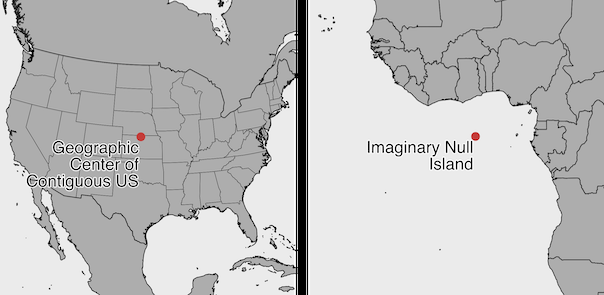
\includegraphics[width=\linewidth, height=0.52\textheight, keepaspectratio]{images/fig_3_4_null_island.png}\\[0.15cm]
{\fontsize{6.8pt}{8pt}\selectfont \textcolor{navyMuted}{\textit{Hình 3.4: Bẫy tâm địa lý Kansas (trái) \& Null Island tọa độ (0,0) (phải).}}}
\end{column}
\end{columns}
\slidenumber{12}
\end{frame}

% ==================== SLIDE 15: DỮ LIỆU THÔ ====================
\begin{frame}[plain, t]
\slideheader{Chương 4 • Dữ Liệu Thô, Làm Sạch}{Thực Trạng Phũ Phàng Của Bảng Dữ Liệu Thô}
\begin{columns}[T]
\begin{column}{0.52\textwidth}
{\fontsize{8.2pt}{10.5pt}\selectfont
\textbf{1. Trùng lặp \& Khoảng trắng thừa (Whitespaces)}
\begin{itemize}\setlength{\itemsep}{2pt}
    \item Khoảng trắng vô hình ở cuối chuỗi (\texttt{"Brazil "} vs \texttt{"Brazil"}) khiến máy tính coi đây là 2 quốc gia khác nhau khi gom nhóm.
\end{itemize}

\vspace{0.12cm}
\textbf{2. Tách đơn vị đo khỏi cột số}
\begin{itemize}\setlength{\itemsep}{2pt}
    \item Xóa bỏ ký hiệu \$, dấu phẩy, \texttt{kg}, \% (\texttt{282,805a} $\rightarrow$ \texttt{282805}) để đưa văn bản (căn trái) về số thực thụ (căn phải).
\end{itemize}

\vspace{0.12cm}
\textbf{3. Cẩn trọng khi Tìm \& Thay thế (Find \& Replace)}
\begin{itemize}\setlength{\itemsep}{2pt}
    \item \textbf{Bài toán:} 169 thị trấn Connecticut thừa chữ \texttt{"town"} (\texttt{Hartford town}, \texttt{Newtown town}).
    \item \textcolor{accentRed}{\textbf{Bẫy:}} Thay \texttt{"town"} $\rightarrow$ \texttt{Newtown} bị biến thành \texttt{New}!
    \item \textbf{Chuẩn:} Phải tìm chính xác chuỗi \textbf{\texttt{" town"} (có dấu cách phía trước)}.
\end{itemize}
}
\end{column}
\begin{column}{0.44\textwidth}
\centering
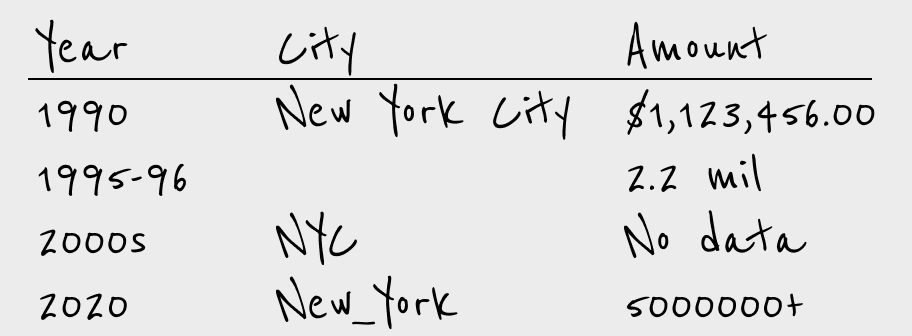
\includegraphics[width=\linewidth, height=0.52\textheight, keepaspectratio]{images/fig_4_1_messy_data.png}\\[0.15cm]
{\fontsize{6.8pt}{8pt}\selectfont \textcolor{navyMuted}{\textit{Hình 4.1: Bản phác thảo các lỗi định dạng kinh điển của dữ liệu thô.}}}
\end{column}
\end{columns}
\slidenumber{15}
\end{frame}
% ==================== SLIDE 17: TRANSPOSE, SPLIT & COMBINE ====================
\begin{frame}[plain, t]
\slideheader{Chương 4 • Kỹ Thuật Làm Sạch}{Tái Cấu Trúc Bảng: Transpose, Split \& Combine}
\begin{columns}[T]
\begin{column}{0.48\textwidth}
\calloutbox[\linewidth]{1. Xoay Trục Dữ Liệu: Transpose (Hàng $\leftrightarrow$ Cột)}{
    \textbf{Mâu thuẫn góc nhìn:}
    \begin{itemize}\setlength{\itemsep}{2pt}
        \item Khi trình bày \textbf{Bảng (Table)} cho người đọc: Thời gian xếp \textbf{nằm ngang} theo cột (\texttt{2000 | 2010 | 2020}).
        \item Khi vẽ \textbf{Biểu đồ đường}: Phần mềm yêu cầu thời gian phải chạy \textbf{thẳng đứng} theo cột đầu tiên từ trên xuống dưới.
    \end{itemize}
    $\rightarrow$ Kỹ thuật \textbf{Transpose} giúp đảo ngược ma trận Hàng $\leftrightarrow$ Cột tức thời mà không cần nhập lại dữ liệu.
}
\end{column}
\begin{column}{0.48\textwidth}
\calloutbox[\linewidth]{2. Tách Cột \& Gộp Cột }{
    \textbf{Tách cột:}
    \begin{itemize}\setlength{\itemsep}{1.5pt}
        \item Khi nhiều thực thể bị nhét chung vào 1 ô:
        \item \texttt{300 Summit St, Hartford CT--06106}
        \item Dùng dấu phân cách (\texttt{,}, khoảng trắng, \texttt{--}) tách thành 4 cột riêng: \texttt{Street | City | State | Zip}.
    \end{itemize}
    \vspace{0.08cm}
    \textbf{Gộp cột :}
    \begin{itemize}\setlength{\itemsep}{1.5pt}
        \item Ngược lại, khi nạp vào công cụ bản đồ, nối các cột địa chỉ rời rạc thành một chuỗi duy nhất có dấu phẩy phân cách.
    \end{itemize}
}
\end{column}
\end{columns}
\slidenumber{17}
\end{frame}

% ==================== SLIDE 18: CLUSTERING ====================
\begin{frame}[plain, t]
\slideheader{Chương 4 • Kỹ Thuật Làm Sạch}{Gom Cụm Chuẩn Hóa Tên Gọi}
\begin{columns}[T]
\begin{column}{0.51\textwidth}
{\fontsize{8.2pt}{10.5pt}\selectfont
\textbf{Thực tế dữ liệu viện trợ Mỹ:}
\begin{itemize}\setlength{\itemsep}{2pt}
    \item Chỉ riêng 2 quốc gia Triều Tiên và Hàn Quốc nhưng xuất hiện tới \textbf{26 cách viết khác nhau}:
    \texttt{Korea, N}, \texttt{Korea-North}, \texttt{SouthKorea}, \texttt{So Korea}, \texttt{Korea, South}...
    \item Cơ quan tài trợ sai chính tả: \texttt{Dept of Agriculture}, \texttt{Department of Argic}...
\end{itemize}

\vspace{0.12cm}
\textbf{Thuật toán Gom cụm thông minh:}
\begin{itemize}\setlength{\itemsep}{2pt}
    \item \textbf{Key Collision:} Chuẩn hóa chữ hoa/thường, xóa dấu câu, sắp xếp lại từ khóa. Tốc độ rất cao, quét tập dữ liệu lớn.
    \item \textbf{Nearest Neighbor:} Tính khoảng cách chỉnh sửa giữa các chuỗi để bắt các lỗi chính tả tinh vi.
\end{itemize}
}
\end{column}
\begin{column}{0.45\textwidth}
\centering
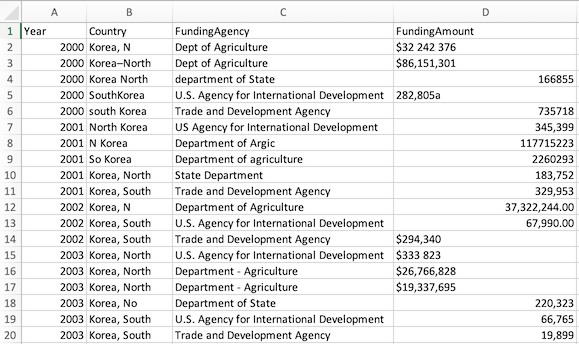
\includegraphics[width=\linewidth, height=0.25\textheight, keepaspectratio]{images/fig_4_11_korea_raw.png}\\[0.1cm]
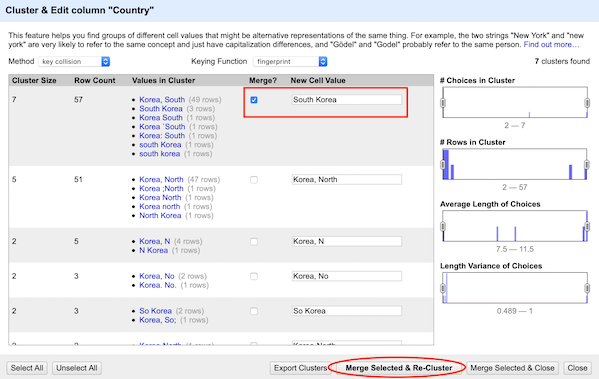
\includegraphics[width=\linewidth, height=0.26\textheight, keepaspectratio]{images/fig_4_18_korea_cluster.png}\\[0.1cm]
{\fontsize{6.5pt}{7.8pt}\selectfont \textcolor{navyMuted}{\textit{Hình 4.11: Dữ liệu thô lộn xộn \& Hình 4.18: Giao diện gom cụm về 1 tên.}}}
\end{column}
\end{columns}
\slidenumber{18}
\end{frame}

% ==================== SLIDE 19: CHUYỂN TIẾP CHƯƠNG 5 ====================

% ==================== SLIDE 20: MEAN VS. MEDIAN ====================
\begin{frame}[plain, t]
\slideheader{Chương 5 • Ngôn Từ Chuẩn Xác}{Trung Bình (Mean) vs. Trung Vị (Median)}
\begin{columns}[T]
\begin{column}{0.54\textwidth}
{\fontsize{7.8pt}{9.8pt}\selectfont
\textbf{Chọn sai đại lượng sẽ bóp méo hoàn toàn câu chuyện:}
\begin{itemize}\setlength{\itemsep}{1pt}
    \item \textbf{Mean (Trung bình):} Rất nhạy cảm, dễ bị kéo lệch bởi ngoại lai.
    \item \textbf{Median (Trung vị):} Giá trị chính giữa, kháng nhiễu tuyệt đối.
\end{itemize}
}
\calloutbox[\linewidth]{1. Thay Đổi Phần Trăm (Percent Change)}{
    Biến thiên tương đối so với giá trị ban đầu:\\[0.12cm]
    \centering
    $\boldsymbol{\Delta\% = \dfrac{V_{\text{mới}} - V_{\text{cũ}}}{|V_{\text{cũ}}|} \times 100\%}$
}

\vspace{0.12cm}
\calloutbox[\linewidth]{2. Chênh Lệch Điểm Phần Trăm (Percentage Point)}{
    Phép trừ số học giữa hai số tỷ lệ \%:\\[0.12cm]
    \centering
    \textbf{Điểm \% = Tỷ lệ Mới $-$ Tỷ lệ Cũ}
}
\end{column}
\begin{column}{0.42\textwidth}
\centering
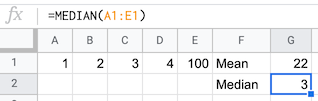
\includegraphics[width=\linewidth, height=0.40\textheight, keepaspectratio]{images/fig_5_1_median_vs_mean.png}\\[0.08cm]
{\fontsize{6.5pt}{7.5pt}\selectfont \textcolor{navyMuted}{\textit{Hình 5.1: Minh họa Mean nhảy vọt lên 22 trong khi Median giữ vững ở 3.}}}
\end{column}
\end{columns}
\slidenumber{20}
\end{frame}


% ==================== SLIDE 22: TƯƠNG QUAN ≠ NHÂN QUẢ ====================
\begin{frame}[plain, t]
\slideheader{Chương 5 • Ngôn Từ Chuẩn Xác}{Tương Quan Không Đồng Nghĩa Với Nhân Quả}
\begin{columns}[T]
\begin{column}{0.54\textwidth}
{\fontsize{8.2pt}{10.5pt}\selectfont
\textbf{Cực kỳ thận trọng với các động từ mang tính áp đặt:}
\textit{``dẫn đến'' (leads to)}, \textit{``thúc đẩy'' (promotes)}, \textit{``gây ra'' (causes)}.

\begin{itemize}\setlength{\itemsep}{2pt}
    \item \textbf{Tương quan (Correlation):} Hai biến số cùng biến thiên trên biểu đồ (ví dụ: tuổi thọ càng cao thì tỷ lệ sinh càng thấp).
    \item \textbf{Nhân quả (Causation):} Biến độc lập trực tiếp tạo ra sự thay đổi ở biến phụ thuộc.
\end{itemize}

\vspace{0.12cm}
\textbf{3 bước bắt buộc để khẳng định Quan hệ Nhân quả:}
\begin{enumerate}\setlength{\itemsep}{1.5pt}
    \item Chứng minh có \textbf{tương quan thống kê rõ rệt}.
    \item Xây dựng \textbf{lý thuyết cơ chế tác động} thuyết phục.
    \item \textbf{Cô lập hoàn toàn mọi biến gây nhiễu (Confounding variables)} -- yếu tố ẩn tác động đồng thời lên cả hai biến.
\end{enumerate}
}
\end{column}
\begin{column}{0.42\textwidth}
\centering
\begin{tikzpicture}[scale=0.9]
    \node[draw=navyMain, fill=boxBg, rounded corners=4pt, align=center, font=\scriptsize\bfseries] (C) at (0, 2.0) {Biến Gây Nhiễu Ẩn\\(Confounding C)};
    \node[draw=navyMain, fill=white, rounded corners=4pt, align=center, font=\scriptsize\bfseries] (A) at (-1.8, 0) {Biến A\\(Quan sát)};
    \node[draw=navyMain, fill=white, rounded corners=4pt, align=center, font=\scriptsize\bfseries] (B) at (1.8, 0) {Biến B\\(Quan sát)};
    \draw[{Latex[length=2mm]}-{Latex[length=2mm]}, dashed, line width=1.1pt, accentRed] (A) -- (B);
    \node[font=\tiny\bfseries, color=accentRed] at (0, -0.55) {Tương quan biểu kiến};
    \draw[-{Latex[length=2.5mm]}, line width=1.2pt, navyMain] (C) -- (A) node[midway, left, font=\tiny] {Tác động};
    \draw[-{Latex[length=2.5mm]}, line width=1.2pt, navyMain] (C) -- (B) node[midway, right, font=\tiny] {Tác động};
\end{tikzpicture}\\[0.15cm]
{\fontsize{6.8pt}{8pt}\selectfont \textcolor{navyMuted}{\textit{Sơ đồ tam giác: A và B tương quan chỉ vì cùng bị C chi phối!}}}
\end{column}
\end{columns}
\slidenumber{22}
\end{frame}
% ==================== SLIDE 24: CHUẨN HÓA KHÁC ====================
\begin{frame}[plain, t]
\slideheader{Chương 5 • Chuẩn Hóa Dữ Liệu}{Các Phương Pháp Chuẩn Hóa \& Ngoại Lệ}
\begin{columns}[T]
\begin{column}{0.51\textwidth}
{\fontsize{8.2pt}{10.5pt}\selectfont
\textbf{Các kỹ thuật chuẩn hóa chuyên sâu khác:}
\begin{itemize}\setlength{\itemsep}{2pt}
    \item \textbf{1. Điều chỉnh theo lạm phát:}
    Không thể so thu nhập \$10.000 năm 1970 với năm 2020. Phải quy đổi từ số danh nghĩa sang sức mua thực tế.
    \item \textbf{2. Điều chỉnh theo mùa vụ:}
    Loại bỏ biến động chu kỳ tự nhiên (du lịch mùa hè, bán lẻ dịp Giáng sinh) để thấy xu hướng thực chất.
    \item \textbf{3. Chỉ số hóa:}
    Đưa các biến có đơn vị khác nhau về cùng mốc chuẩn Base 100 hoặc độ lệch chuẩn.
\end{itemize}
}
\end{column}
\begin{column}{0.45\textwidth}
\calloutbox[\linewidth]{Khi Nào KHÔNG CẦN Chuẩn Hóa?}{
    Khi biến số bản thân nó đã là một \textbf{đại lượng đo lường trên thang quy chiếu chung}:\\[0.1cm]
    • \textbf{Độ tuổi trung vị (Median Age):} Con người ở mọi thành phố đều sống trong thang tuổi 0--120, có thể so sánh trực tiếp.\\
    • \textbf{Thu nhập hộ gia đình trung vị:} Xét trong cùng 1 năm và 1 đơn vị tiền tệ có thể đối chiếu giữa các vùng mà không cần chia theo đầu người!
}
\end{column}
\end{columns}
\slidenumber{24}
\end{frame}

% ==================== SLIDE 25: SELECTION & NON-RESPONSE ====================
\begin{frame}[plain, t]
\slideheader{Chương 5 • Bẫy Chọn Mẫu}{Thiên Vị Chọn Mẫu \& Không Phản Hồi}
\begin{columns}[T]
\begin{column}{0.52\textwidth}
{\fontsize{8.5pt}{11.5pt}\selectfont
\vspace{0.12cm}
\textbf{1. Thiên vị chọn mẫu (Selection Bias)}
\begin{itemize}\setlength{\itemsep}{2pt}
    \item Mẫu được chọn khác biệt có hệ thống so với tổng thể chung.
\end{itemize}

\vspace{0.22cm}
\textbf{2. Thiên vị không phản hồi (Non-response Bias)}
\begin{itemize}\setlength{\itemsep}{2pt}
    \item Nhóm từ chối hoặc không phản hồi có đặc tính khác biệt rõ rệt với nhóm tham gia trả lời.
\end{itemize}

\vspace{0.22cm}
\textbf{3. Thiên vị tự lựa chọn (Self-selection Bias)}
\begin{itemize}\setlength{\itemsep}{2pt}
    \item Xảy ra khi đánh giá hiệu quả chương trình nơi người tham gia \textbf{tự nguyện đăng ký} (giảm cân, học bổng).
\end{itemize}
}
\end{column}
\begin{column}{0.44\textwidth}
\centering
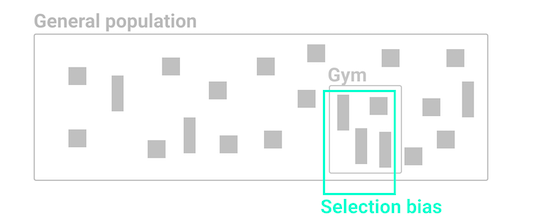
\includegraphics[width=\linewidth, height=0.48\textheight, keepaspectratio]{images/fig_5_2_selection_bias.png}\\[0.1cm]
{\fontsize{6.5pt}{7.5pt}\selectfont \textcolor{navyMuted}{\textit{Hình 5.2: Khung Gym chỉ toàn người cao so với tổng thể chung.}}}
\end{column}
\end{columns}
\slidenumber{25}
\end{frame}
\end{document}